\section{Creating Rapport Agents using Hybrid Approaches}

Recently, researchers are exploring hybrid agents that combine the advantage of rule-based systems to define high-level interaction rules that are triggered by simpler perceptual states and data-driven models to generate behaviour according to more complex situations that may emerge during interactions.

Pedro Sequeira et. al. proposes the usage of mock-up studies and the previously mentioned restricted-perception \ac{WoZ} (Section~\ref{subsec:woz}) to develop a Hybrid Controller that takes advantage of rule-based systems and \ac{ML}-based systems in a tutoring scenario~\cite{Sequeira2016}. Following Figure~\ref{fig:RestrictedPerception_DesignProcess}, the inherent agent's limitations are defined in the \textit{Task AI} to be used on the restricted-perception \ac{WoZ} Studies. The hybrid controller is based on the expert knowledge and the \ac{WoZ} data collected during the previous stage, and is responsible for deciding when and which behaviour to trigger. For example, a rule-based component would trigger a summarisation of the main achievements during the game and another \ac{ML}-based component would trigger actions that were learnt during the restricted-perception \ac{WoZ} studies (recall that the wizards controls ``which interaction behaviour should be triggered and when to trigger it''~\cite{Sequeira2016}). In the last stage, \textit{Strategy Refinement}, \ac{HRI} researchers assess the agent's performance and refines the controller if necessary for situations that may not have been properly learned or, for situations that require more relevant information.

\begin{figure}[H]
	\centering
	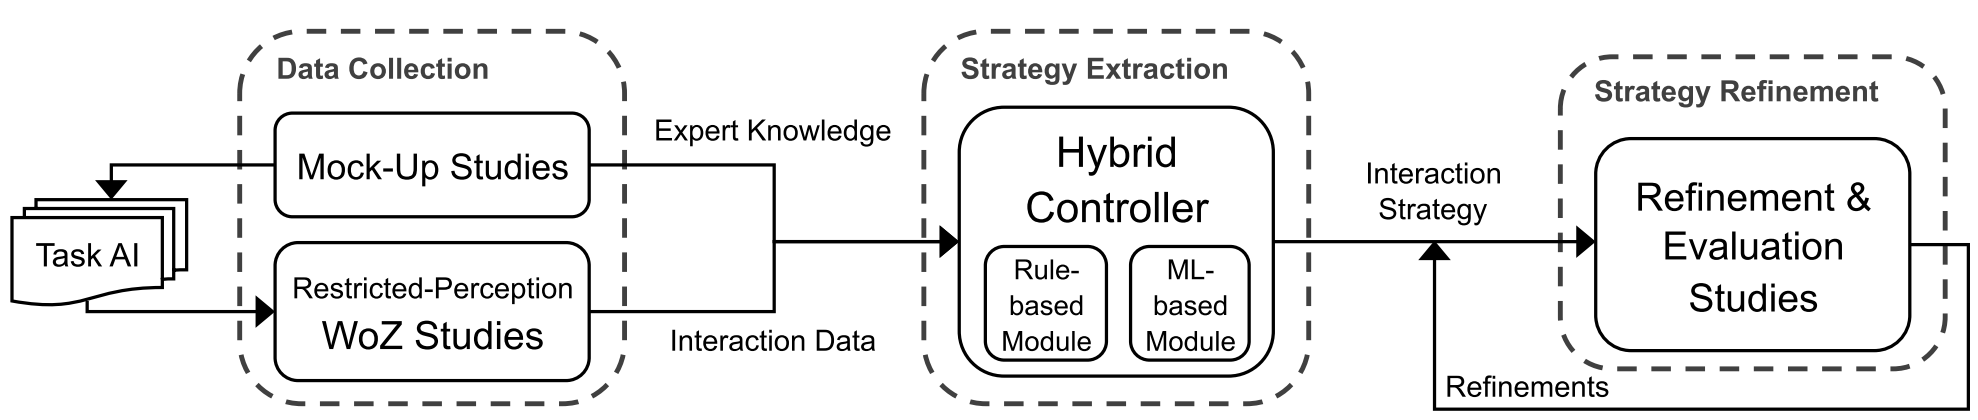
\includegraphics[width=0.85\textwidth]{images/RestrictedPerception_DesignProcess.png}
	\caption{Restricted-perception \ac{WoZ} study methodology. From~\cite{Sequeira2016}.}
	\label{fig:RestrictedPerception_DesignProcess}
\end{figure}




\subsubsection{Virtual Rapport 2.0} \hspace*{\fill} \\
\label{sub:sec:virtualrapport2}

Huang et al., developed a short-term rapport agent to enhance mutual attention and coordination using backchannels through a data-driven approach that takes into account context-specific response models in a dyadic conversational setting~\cite{Buschmeier2011}. The model determines the best suitable timings to generate specific backchannel behaviours and turn-taking opportunities according to the perceptual state observed.

%%%%%%%%%%%%%%%%%%%%%%%%%%%%%%%%%%%%%%%%%%%%%%%%%%%%%%%%%%%%%%%%%%%%%%%%%%%%%%%%%%%%%

\paragraph{\textbf{System description}}

Following Figure~\ref{fig:virtualrapport2System}, the system contains the following modules:
\begin{itemize}
	\item \textbf{\textit{Perception}}: analyses human speaker's behaviour in real time;
	\item \textbf{\textit{Response Models}}: predicts timing of backchannel feedback and end-of-turn opportunities in real time using information from the environment and from the agent itself. It also decides which behaviour to generate;
	\item \textbf{\textit{Generation}}: generates the output from the response models;	
	\item \textbf{\textit{Consensus Data}}: contains data collected from Rapport 06-07 dataset and Self-disclosure data-set (\url{http://rapport.ict.usc.edu}) using \ac{PCS}. The data contains dyadic interactions between a human speaker telling a story and human silent listener.
\end{itemize}

\begin{figure}[hbt]
  \centering
  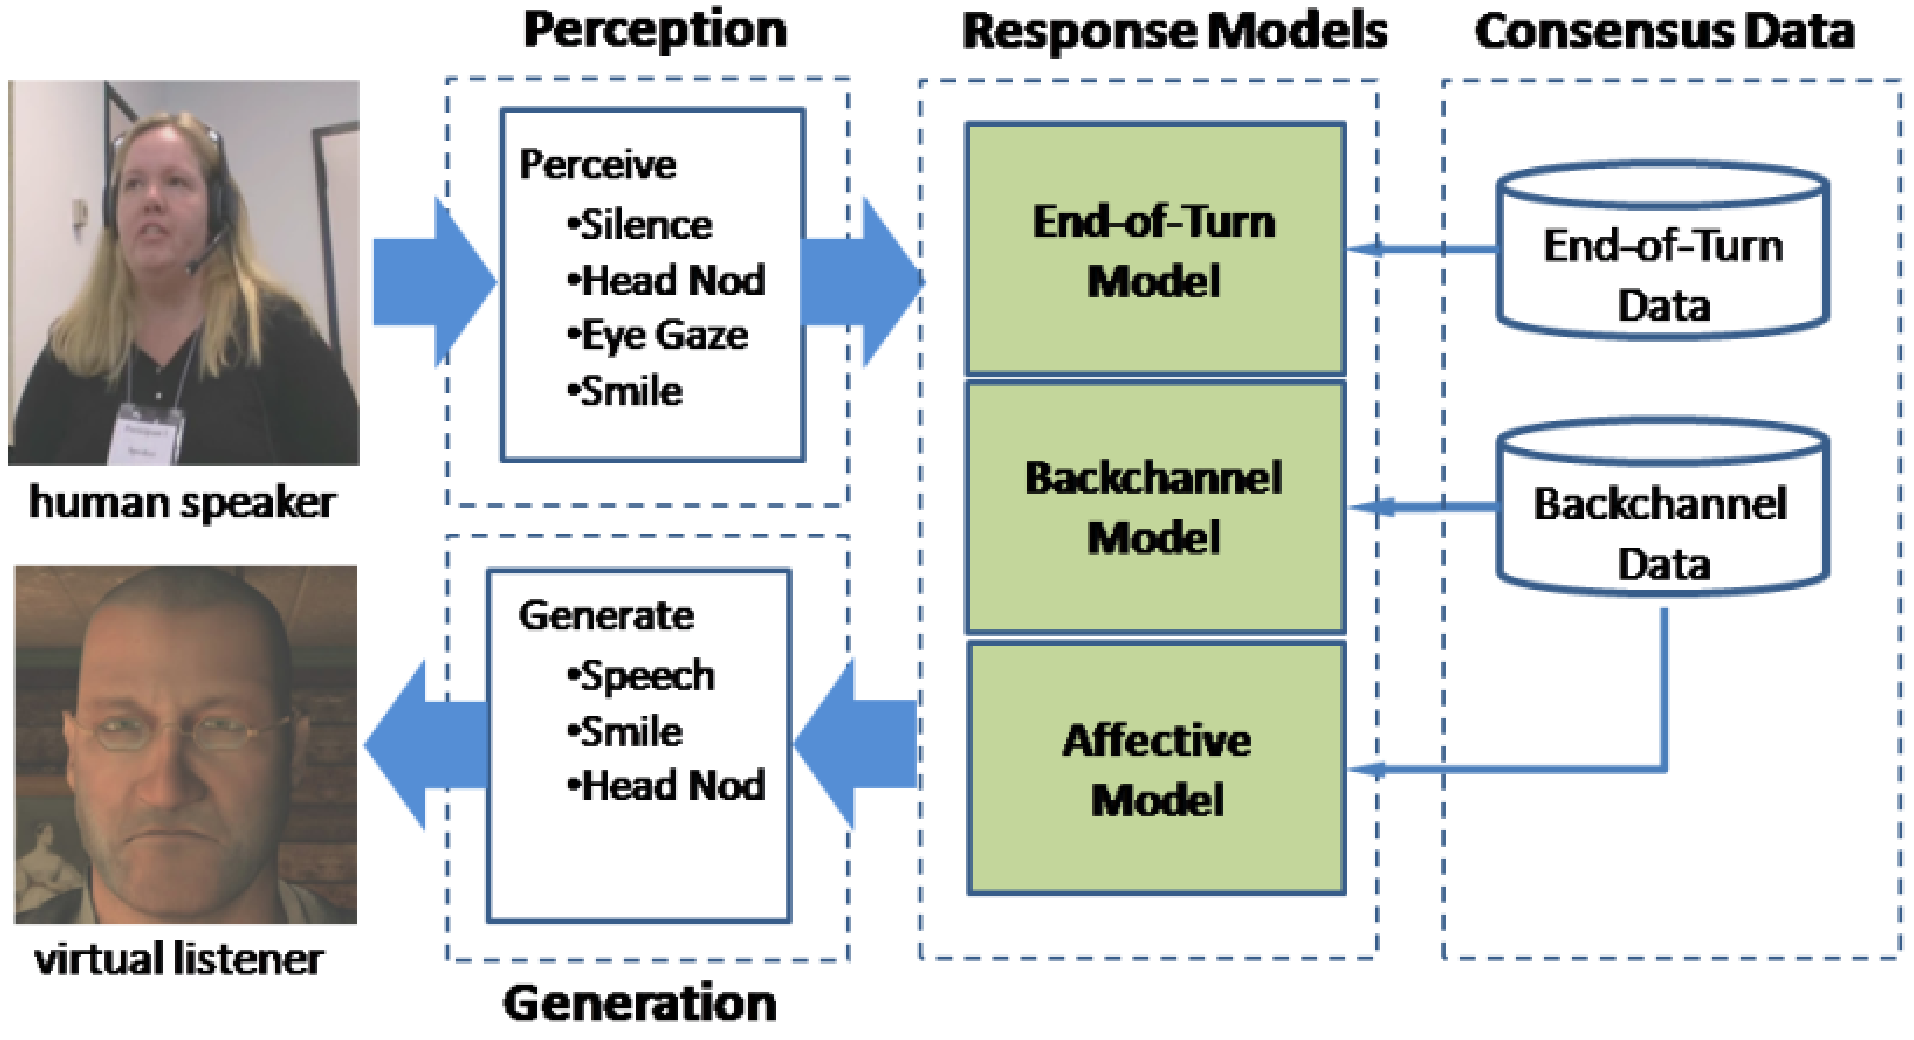
\includegraphics[width=0.8\textwidth]{images/VirtualRapport2_System.png}
  \caption{Architecture of Virtual Rapport 2.0: The \textit{Perception} module analyses human behaviour in real time. \ac{PCS} data is used to create the \textit{Response Models} module. Lastly, the output of the models is generated by the \textit{Generation} module. From~\cite{Buschmeier2011}.}
  \label{fig:virtualrapport2System}
\end{figure} 

As depicted in Figure \ref{fig:virtualrapport2System} there are three models in the \textit{Response Models} module: \textit{End-of-turn}, \textit{Backchannel}, and \textit{Affective}.

The first model, \textit{end-of-turn}, using a rule-based approach, identifies turn-taking opportunities by analysing the current speaker's non-verbal behaviours. For example, if the human interrupts the virtual agent, the agent stops, yields his turn and, says ``I am sorry, keep going'' while showing a facial expression~\cite{Buschmeier2011}.

The second model, \textit{Backchannel}, is \ac{ML}-based (using forward-only inference \ac{CRF} for real-time predictions) and trained using the Rapport 06-07 dataset. It is capable of predicting when and how to give non-verbal feedback.

The last model, \textit{Affective}, analyses facial feature points in real time and detects whenever the speaker is smiling.
 
During the interaction, the three response models are used in conjunction to decide whenever it is appropriate to generate a backchannel. If the speaker is smiling (according to the \textit{Affective} model) and if it is a good opportunity to generate a backchannel (according to the \textit{Backchannel} model) then a head nod (one of the three identified in their studies) is generated accompanied by a smile.

%%%%%%%%%%%%%%%%%%%%%%%%%%%%%%%%%%%%%%%%%%%%%%%%%%%%%%%%%%%%%%%%%%%%%%%%%%%%%%%%%%%%%%%%

\paragraph{\textbf{Evaluation}}
The developed virtual agent interacted with the human subjects in a interview environments in which the former was the interviewer and the later the interviewed. With the goal of comparing the developed system with the previous version~\cite{Gratch2006}, the evaluation measured the following dimensions: rapport (five-item social presence scale~\cite{Bailenson2001}), overall naturalness, backchannel feedback and end-of-turn prediction.


%%%%%%%%%%%%%%%%%%%%%%%%%%%%%%%%%%%%%%%%%%%%%%%%%%%%%%%%%%%%%%%%%%%%%%%%%%%%%%%%%%%%%%%%

\paragraph{\textbf{Discussion}}
The results demonstrates a significant improvement over the previous version. Over 90\% of the users preferred the Virtual Rapport 2.0 rapport agent over the previous rule-based system~\cite{Gratch2006, Morency2008}. The timing's precision and recall are much better, leading to a better synchronism and perceived naturalness from the user during the interaction. According to the authors, the data-driven design, the much richer set of emotions capable of mimicking smiles, and the generation of more natural head gestures might explain the overall better results on the stronger feelings of rapport.

To conclude the most relevant aspects of the system are:
\begin{itemize}
	\item Corpus based approach;
	\item Identification of different head nods patterns;
	\item Duality of \ac{ML}-bases decision and smile to generate backchannel behaviour;
	\item Creative strategy for handling interruptions.
\end{itemize}
\subsubsection{\acl{SAL}} \hspace*{\fill} \\
\label{subsec:AutonomousSensitiveArtificialListeners}

Schröder et al. developed a virtual agent integrated in SEMAINE~\cite{Schroder2010} called \ac{SAL} that has the required capabilities to sustain conversational dialogues and be a good listener~\cite{Schroder2012}.

\paragraph{\textbf{System Description}}

Following the representation of the \ac{SAL} system in Figure~\ref{fig:sensitiveAgent}, the most relevant components are: \textit{Feature extractors}, \textit{Analysers}, \textit{Interpreters}, \textit{Action proposers}, and \textit{Action selection}. The \textit{Feature extractors} component extracts several features such as head gestures, facial features, emotions and, most of all, acoustic features. These features are later analysed by the \textit{Analysers} and \textit{Interpreters} components. The former component analyses non-verbal behaviours and speaker's emotions to produce an estimate of the information's reliability. The later component, given the information available, returns the best state representation for the user, dialogue and agent. Following this, several \textit{Action proposers} will propose an action, in parallel, given previous information. Following, the \textit{Action selection} component selects the action with the highest estimated quality, and lastly, the \textit{Behaviour generator} generates the desired action (utterances and facial animations).

\vspace{-3mm}
\begin{figure}
	\centering
	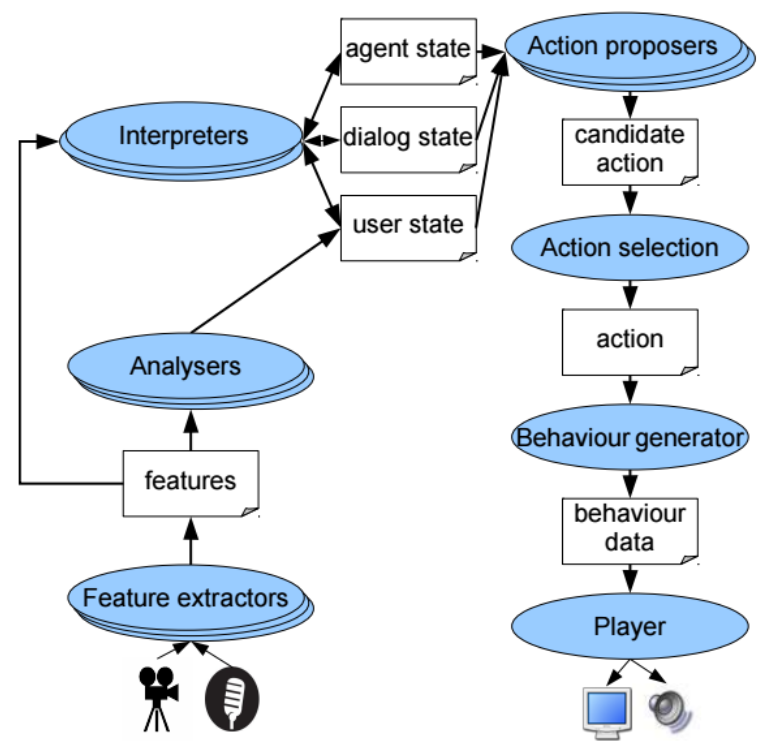
\includegraphics[width=0.5\textwidth]{images/SensitiveAgent.png}
	\caption{\acl{SAL} conceptual architecture. From~\cite{Schroder2012}.}
	\label{fig:sensitiveAgent}
\end{figure}
\vspace{-7mm}

The agent is capable of identifying whether it should be in listener or in speaker mode. This is relevant as the \textit{Action selection} component gives more priority over speaker's actions. An example speaker action would be  saying ``Well?'' or ``Go on, tell me your news!'' after a long pause. In addition, in listener mode, the \textit{Action selection} component chooses the most appropriate backchannel to be produced according to the emotions and interest level estimated from the user.

\paragraph{\textbf{Evaluation}}

The objective was to evaluate if emotion-related abilities influence the quality of human interactions. Firstly the users, with minimal \ac{HRI} experience, receive a introductory briefing on the available personalities they can interact with (4 in total). Then, they can interact twice with each available personality one with the expressive agent, the other with the affective features of the output disabled (randomly). The user interacts with the \ac{SAL} agent's presented in a computer screen (only the face is rendered), using the available cameras and microphones.

\paragraph{\textbf{Discussion}}
There is evidence that expressive abilities may substantially impact the interactions between humans and agents by denoting that flow and perceived engagement was much higher in the emotional \ac{SAL} than in the control environment. Compared with previous described systems, it is one of the most complete models for managing backchannels and turn taking strategies, however, as stated previously in Section~\ref{subsec:Rapport}, attentiveness and coordination are not enough to build rapport, it is also necessary to stimulate positivity which this system does not cover. To conclude, the most relevant aspects of the systems are:

\begin{itemize}
	\item Generate good listeners without understanding semantically what it is being said;
	\item Parallel independent action proposers that uses both rule and \ac{ML} approaches;
	\item Dedicated dialogue management models;
	\item Covers several users affective states by modelling distinct characters.
\end{itemize}